\chapter{反函数和反三角函数}
1.导数与反函数\\
如果$f$在其定义域$(a,b)$上可导且满足以下条件中的任意一条:\\
(1)对于所有的在$(a,b)$中的$x$, $f'(x)>0$;\\
(2)对于所有的在$(a,b)$中的$x$, $f'(x)<0$;\\
(3)对于所有的在$(a,b)$中的$x$, $f'(x)\geqslant 0$且对于有限个数的$x$, $f'(x)=0$;\\
(4)对于所有的在$(a,b)$中的$x$, $f'(x)\leqslant 0$且对于有限个数的$x$, $f'(x)=0$.\\
则$f$有反函数.\\[2ex]

反函数的导数:
\begin{center}
\framebox{如果$\displaystyle y=f^{-1}(x)$, 则$\displaystyle\frac{\dif y}{\dif x}=\frac{1}{f'(y)}=\frac{1}{f'(f^{-1}(x))}$}\\[1ex]
\end{center}
例.\\
\phantom{例}$h(x)=x^3$, 如果$y=h^{-1}(x)$, 求$\displaystyle\frac{\dif y}{\dif x}$\\
推导过程:\\
$\displaystyle\frac{\dif y}{\dif x}=\frac{1}{f'(y)}=\frac{1}{(y^3)'}=\frac{1}{3y^2}$\\
$\displaystyle y=h^{-1}(x)=x^{\frac{1}{3}}$\\
$\displaystyle\therefore\frac{\dif y}{\dif x}=\frac{1}{3y^2}=\frac{1}{3x^{\frac{2}{3}}}$\\[2ex]

2.反三角函数\\
(1)$\sin^{-1}$是奇函数; 其定义域为$[-1,1]$, 值域为$\displaystyle[-\frac{\pi}{2},\frac{\pi}{2}]$\\[1ex]
(2)$\displaystyle\frac{\dif }{\dif x}\sin^{-1}(x)=\frac{1}{\sqrt{1-x^2}}$, 其中$-1<x<1$.\\[1ex]
如图:
\begin{figure}[H]
\centering
	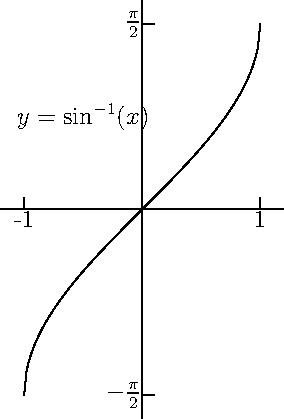
\includegraphics{asin.pdf}
\end{figure}
例.\\
\phantom{例}$\displaystyle\frac{\dif}{\dif x}\sin^{-1}(x)$\\
推导过程:\\
$\displaystyle\because y=\sin^{-1}(x)$, 即$x=\sin(y)$;
$\displaystyle\therefore\frac{\dif}{\dif x}\sin^{-1}(x)=\frac{1}{f'(y)}=\frac{1}{\cos(y)}$\\
$\displaystyle\because\cos(y)=\pm\sqrt{1-\sin^2y}$, 并且$\sin^{-1}(x)$斜率在$(-1,1)$上恒为正\\
$\displaystyle\therefore\cos(y)=\sqrt{1-\sin^2y}=\sqrt{1-x^2}$\\
$\displaystyle\therefore\frac{\dif}{\dif x}\sin^{-1}(x)=\frac{1}{\cos(y)}=\frac{1}{\sqrt{1-x^2}}$\\[1ex]

(3)$\cos^{-1}$既不是偶函数也不是奇函数; 其定义域为$[-1,1]$, 值域为$[0,\pi]$.\\[1ex]
(4)$\displaystyle\frac{\dif }{\dif x}\cos^{-1}(x)=-\frac{1}{\sqrt{1-x^2}}$, 其中$-1<x<1$.\\[1ex]
如图:
\begin{figure}[H]
\centering
	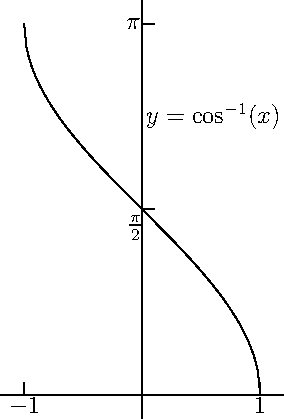
\includegraphics{acos.pdf}
\end{figure}
例.\\
\phantom{例}$\displaystyle\frac{\dif}{\dif x}\cos^{-1}(x)$\\
推导过程:\\
$\displaystyle\because y=\cos^{-1}(x)$, 即$x=\cos(y)$\\
$\displaystyle\therefore\frac{\dif}{\dif x}\cos^{-1}(x)=\frac{1}{f'(y)}=-\frac{1}{\sin(y)}$\\
$\displaystyle\because\sin(y)=\pm\sqrt{1-\cos^2y}$, 并且$\cos^{-1}(x)$在$(-1,1)$上恒为负\\
$\displaystyle\therefore\sin(y)=\sqrt{1-\cos^2y}=\sqrt{1-x^2}$\\
$\displaystyle\therefore\frac{\dif}{\dif x}\cos^{-1}(x)=-\frac{1}{\sin(y)}=-\frac{1}{\sqrt{1-x^2}}$\\[1ex]

(5)$\tan^{-1}$是奇函数; 其定义域是$\mathbb{R}$且值域是$\displaystyle(-\frac{\pi}{2},\frac{\pi}{2})$.\\[1ex]
(6)对于所有的实数$x$, $\displaystyle\frac{\dif }{\dif x}\tan^{-1}(x)=\frac{1}{1+x^2}$.\\[1ex]
如图:
\begin{figure}[H]
\centering
	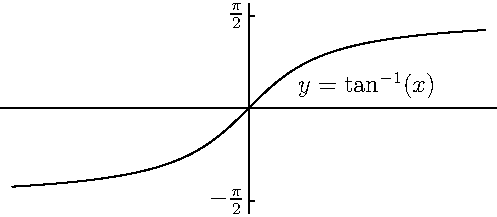
\includegraphics{atan.pdf}
\end{figure}
例.\\
\phantom{例}$\displaystyle\frac{\dif}{\dif x}\tan^{-1}(x)$\\
推导过程:\\
$\displaystyle\because y=\tan^{-1}(x)$, 即$x=\tan(y)$\\
$\displaystyle\therefore\frac{\dif}{\dif x}\tan^{-1}(x)=\frac{1}{f'(y)}=\frac{1}{\sec^2y}=\frac{1}{1+\tan^2y}=\frac{1}{1+x^2}$\\[1ex]

(7)$\cot^{-1}$既不是奇函数也不是偶函数; 其定义域为$\mathbb{R}$且值域是$(0,\pi)$\\[1ex]
(8)对于所有的实数$x$, $\displaystyle\frac{\dif }{\dif x}\cot^{-1}(x)=-\frac{1}{1+x^2}$.\\[1ex]
\begin{figure}[H]
\centering
	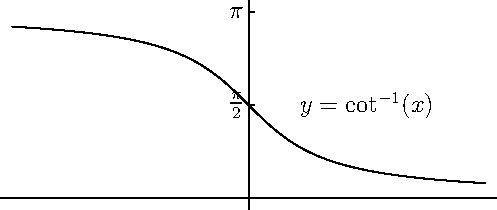
\includegraphics{acot.pdf}
\end{figure}
例.\\
\phantom{例}$\displaystyle\frac{\dif}{\dif x}\cot^{-1}(x)$\\
推导过程:\\
$\displaystyle\because y=\cot^{-1}(x)$, 即$x=\cot(y)$\\
$\displaystyle\therefore\frac{\dif}{\dif x}\cot^{-1}(x)=\frac{1}{f'(y)}=-\frac{1}{\csc^2y}=-\frac{1}{1+\cot^2y}=-\frac{1}{1+x^2}$\\[1ex]

(9)$\sec^{-1}$既不是奇函数也不是偶函数; 其定义域是$(-\infty,-1]\cup[1,\infty)$且值域是$\displaystyle[0,\frac{\pi}{2})\cup(\frac{\pi}{2},\pi]$.\\[1ex]
(10)对于$x>1$或$x<-1$, $\displaystyle\frac{\dif }{\dif x}\sec^{-1}(x)=\frac{1}{|x|\sqrt{x^2-1}}$.\\[1ex]
\begin{figure}[H]
\centering
	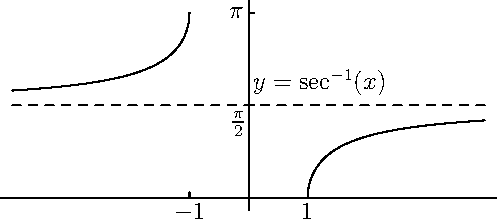
\includegraphics{asec.pdf}
\end{figure}
例.\\
\phantom{例}$\displaystyle\frac{\dif}{\dif x}\sec^{-1}(x)$\\
推导过程:\\
$\displaystyle\because y=\sec^{-1}(x)$, 即$x=\sec(y)$\\
$\displaystyle\therefore\frac{\dif}{\dif x}\sec^{-1}(x)=\frac{1}{f'(y)}=\frac{1}{\tan(y)\sec(y)}$\\
$\displaystyle\because\tan(y)=\pm\sqrt{\sec^2y-1}$, 并且$\sec^{-1}(x)$的斜率在$(-\infty,-1)\cup(1,\infty)$恒为正\\
$\displaystyle\therefore\frac{\dif}{\dif x}\sec^{-1}(x)=\frac{1}{\tan(y)\sec(y)}=\frac{1}{|x|\sqrt{x^2-1}}$\\[1ex]

(11)$\csc^{-1}$是奇函数; 其定义域为$(-\infty,-1]\cup[1,\infty)$且值域是$\displaystyle[-\frac{\pi}{2},0)\cup(0,\frac{\pi}{2}]$.\\[1ex]
(12)对于$x>1$或$x<-1$, $\displaystyle\frac{\dif }{\dif x}\csc^{-1}(x)=-\frac{1}{|x|\sqrt{x^2-1}}$.\\[2ex]
\begin{figure}[H]
\centering
	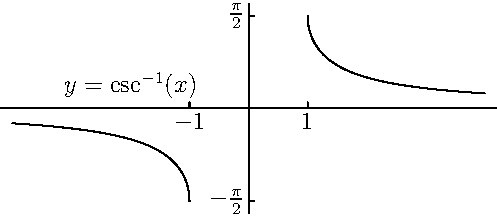
\includegraphics{acsc.pdf}
\end{figure}
例.\\
\phantom{例}$\displaystyle\frac{\dif}{\dif x}\csc^{-1}(x)$\\
推导过程:\\
$\displaystyle\because y=\csc^{-1}(x)$, 即$x=\csc(y)$\\
$\displaystyle\therefore\frac{\dif}{\dif x}\csc^{-1}(x)=\frac{1}{f'(y)}=-\frac{1}{\cot(y)\csc(y)}$\\
$\displaystyle\because\cot(y)=\pm\sqrt{\csc^2y-1}$, 并且$\csc^{-1}(x)$的斜率在$(-\infty,-1)\cup(1,\infty)$上恒为负\\
$\displaystyle\therefore\frac{\dif}{\dif x}\csc^{-1}(x)=-\frac{1}{\cot(y)\csc(y)}=-\frac{1}{|x|\sqrt{x^2-1}}$\\[2ex]

计算反三角函数\\
例1.\\
\phantom{例}$\displaystyle\sin^{-1}(\sin(\frac{13\pi}{10}))$\\
推导过程:\\
$\displaystyle\because\frac{13\pi}{10}$在第三象限\\
$\displaystyle\therefore\sin(\frac{13\pi}{10})<0$且参考角为$(\frac{13\pi}{10}-\pi)=\frac{3\pi}{10}$\\
$\displaystyle\because\sin^{-1}(x)$的值域为$[-\frac{\pi}{2},\frac{\pi}{2}]$\\
$\displaystyle\therefore$当$\sin^{-1}(x)$的$x<0$时, $\sin^{-1}(x)\in[-\frac{\pi}{2},0)$\\
$\displaystyle\therefore$参考角为$\frac{3\pi}{10}$, 并且在区间$[-\frac{\pi}{2},0)$内的角为$-\frac{3\pi}{10}$\\[1ex]

例2.\\
\phantom{例}$\displaystyle\cos^{-1}(\cos(\frac{13\pi}{10}))$\\
推导过程:\\
$\displaystyle\because\frac{13\pi}{10}$在第三象限\\
$\displaystyle\therefore\cos(\frac{13\pi}{10})<0$且参考角为$\frac{3\pi}{10}$\\
$\displaystyle\because\cos^{-1}(x)$的值域为$[0,\pi]$\\
$\displaystyle\therefore$当$\cos^{-1}(x)$的$x<0$时, $\cos^{-1}(x)\in(\frac{\pi}{2},\pi]$\\
$\displaystyle\therefore$参考角为$\frac{3\pi}{10}$, 并且在区间$(\frac{\pi}{2},\pi]$的角为$(\pi-\frac{3\pi}{10})=\frac{7\pi}{10}$\\[1ex]

例3.\\
\phantom{例}$\displaystyle\sin(\sin^{-1}(-\frac{1}{5}))$\\
推导过程:\\
$\displaystyle\because\sin(\sin^{-1}(x))=x$\\
$\displaystyle\therefore\sin(\sin^{-1}(-\frac{1}{5}))=-\frac{1}{5}$\\[1ex]

例4.\\
\phantom{例}$\displaystyle\sin(\cos^{-1}(-\frac{\sqrt{15}}{4}))$\\
推导过程:\\
$\displaystyle\because\cos^{-1}(x)\in[0,\pi]\text{, 并且}-\frac{\sqrt{15}}{4}<0$\\
$\displaystyle\therefore\cos^{-1}(-\frac{\sqrt{15}}{4})$在第二象限\\
$\displaystyle\because\cos(\cos^{-1}(-\frac{\sqrt{15}}{4}))=-\frac{\sqrt{15}}{4}\text{且}\cos^{-1}(-\frac{\sqrt{15}}{4})$在第二象限\\
设$\displaystyle t=\cos^{-1}(x)$, 则:\\
$\displaystyle\sin(t)=\sqrt{1-\cot^2t}=\sqrt{1-\frac{15}{16}}=\frac{1}{4}$\\
即$\displaystyle\sin(\cos^{-1}(-\frac{\sqrt{15}}{4}))=\frac{1}{4}$\\[2ex]

3.反双曲函数\\
(1)$\sinh^{-1}$是奇函数; 其定义域和值域都是$\mathbb{R}$.\\[1ex]
(2)对于所有的实数$x$, $\displaystyle\frac{\dif }{\dif x}\sinh^{-1}(x)=\frac{1}{\sqrt{x^2+1}}$.\\[1ex]
如图.
\begin{figure}[H]
\centering
	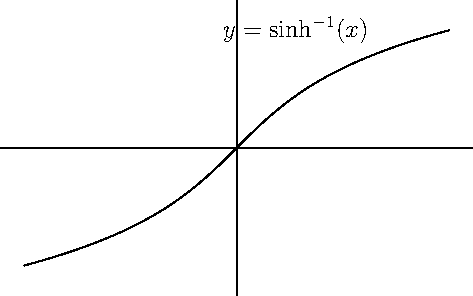
\includegraphics{asinh.pdf}
\end{figure}
例.\\
\phantom{例}$\displaystyle\frac{\dif}{\dif x}\sinh^{-1}(x)$\\
推导过程:\\
$\displaystyle\because y=\sinh^{-1}(x)$, 即$x=\sinh(y)$\\
$\displaystyle\therefore\frac{\dif}{\dif x}\sinh^{-1}(x)=\frac{1}{f'(y)}=\frac{1}{\cosh(y)}$\\
$\displaystyle\because\cosh^2y-\sinh^2y=1$, 并且$\cosh(y)$在$(0,\infty)$上恒为正\\
$\displaystyle\therefore\cosh(y)=\sqrt{1+\sinh^2y}=\sqrt{1+x^2}$\\
$\displaystyle\therefore\frac{\dif}{\dif x}\sinh^{-1}(x)=\frac{1}{\cosh(y)}=\frac{1}{\sqrt{1+x^2}}$\\[1ex]

(3)$\cosh^{-1}$既不是奇函数也不是偶函数; 其定义域是$[1,\infty)$且值域是$[0,\infty)$.\\[1ex]
(4)对于$x>1$, $\displaystyle\frac{\dif }{\dif x}\cosh^{-1}(x)=\frac{1}{\sqrt{x^2-1}}$.\\[1ex]
如图.
\begin{figure}[H]
\centering
	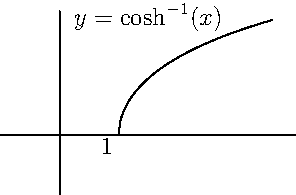
\includegraphics{acosh.pdf}
\end{figure}
例.\\
\phantom{例}$\displaystyle\frac{\dif}{\dif x}\cosh^{-1}(x)$\\
推导过程:\\
$\displaystyle\because y=\cosh^{-1}(x)$, 即$x=\cosh(y)$\\
$\displaystyle\therefore\frac{\dif}{\dif x}\cosh^{-1}(x)=\frac{1}{f'(y)}=\frac{1}{\sinh(y)}$\\
$\displaystyle\because\cosh^2y-\sinh^2y=1$, 并且$\sinh(y)$在$(-\infty,\infty)$上恒为正\\
$\displaystyle\therefore\sinh(y)=\sqrt{\cosh^2y-1}=\sqrt{x^2-1}$\\
$\displaystyle\therefore\frac{\dif}{\dif x}\cosh^{-1}(x)=\frac{1}{\sinh(y)}=\frac{1}{\sqrt{x^2-1}}$

%最后编辑于: 2022-01-23
